\section{Grundlegendes}
\begin{frame}{Warnhinweise}
  \begin{itemize}
    \item 100\% Sicherheit gibt es nicht
    \item Absichern heißt, Angriffe \emph{teurer} zu machen
    \begin{itemize}
    \item Die Kosten für den Angriff\\ müssen den Wert der Daten übersteigen
    \item Ein Angriff darf sich nicht mehr \emph{lohnen}
    \item Problem: Wert wird oft unterschätzt
    \end{itemize}
    \item Was wir hier zeigen, ist ein Anfang
    \begin{itemize}
      \item Hilft dagegen, als ,,Beifang`` zu enden
      \item Gegen gezielte Angriffe -- auch durch Verwechslung -- benötigt es deutlich mehr
    \end{itemize}
  \end{itemize}
\end{frame}

\begin{frame}{Leitfragen}
  \begin{itemize}
    \item \emph{Was} soll sichergestellt werden?
      \begin{itemize}
        \item Eigene Anonymität
        \item Echtheit des Gegenübers (Authentizität)
        \item Unverfälschtheit der Nachricht (Integrität)
        \item Geheimhaltung der Nachricht (Vertraulichkeit)
        \item \ldots
      \end{itemize}
    \item \emph{Wem} vertraut Ihr?
  \end{itemize}
\end{frame}

\begin{frame}{Vertrauen}
  \begin{block}{Woher weiß man, wem man vertrauen kann?}
  \begin{itemize}
    \item Kurze Antwort: weiß man \emph{nicht}
    \item Lange Antwort
    \begin{itemize}
      \item es gibt Fragen, die man stellen kann\ldots
      \item \ldots\ und es gibt das Bauchgefühl
    \end{itemize}
  \end{itemize}
  \end{block}
\end{frame}

\begin{frame}{Welche Fragen kann man stellen?}
  Beispiel: \emph{Wo} sind meine Daten?
  \begin{itemize}
    \item Auf einem Blatt Papier zuhause in meiner Schublade.
    \item Auf meinem Computer:
    \begin{itemize}
      \item Wie gut ist die Software \emph{überprüfbar},\\ die meine Daten verwaltet?
      \begin{itemize}
        \item Open Source (in menschenlesbarer Form öffentlich):\\gut überprüfbar
        \item Closed Source (menschenlesbare Form geheim):\\quasi nicht überprüfbar
      \end{itemize}
    \end{itemize}
    \item In der Cloud
      %TODO: FSF there is no cloud
      \begin{itemize}
        \item \emph{Wer} betreibt einen Dienst?
        \item Womit \emph{verdient} der Betreiber sein \emph{Geld}?
        \item Wem könnten die Daten \emph{nutzen} oder \emph{schaden}?
        \item Was \emph{lernt} der Betreiber über mich?
      \end{itemize}
  \end{itemize}
\end{frame}

\begin{frame}{Meta- und Nutzdaten}
  \begin{itemize}
    \item Meta-/Verbindungsdaten (``Briefumschlag'')
    \begin{itemize}
      \item Absender, Empfänger, Betreff einer E-Mail
      \item Besuch und Aufenthaltsdauer auf einer Webseite
      \item Wer, wann, wie lange mit wem telefoniert
      \item Aufenthaltsort von Mobiltelefonen: Bewegungsprofil!
    \end{itemize}
    \item Nutz-/Inhaltsdaten (``Brief'')
    \begin{itemize}
      \item E-Mail-Text und -Anhänge
      \item Webseiten-Inhalte
      \item Gesprochene Sprache beim Telefonieren
      \item SMS-Inhalt
    \end{itemize}
  \end{itemize}

Metadaten zu verschlüsseln ist nicht möglich,\\ sie zu verschleiern schwierig.
\end{frame}

\begin{frame}{Symmetrische Kryptographie}
  \begin{center}
    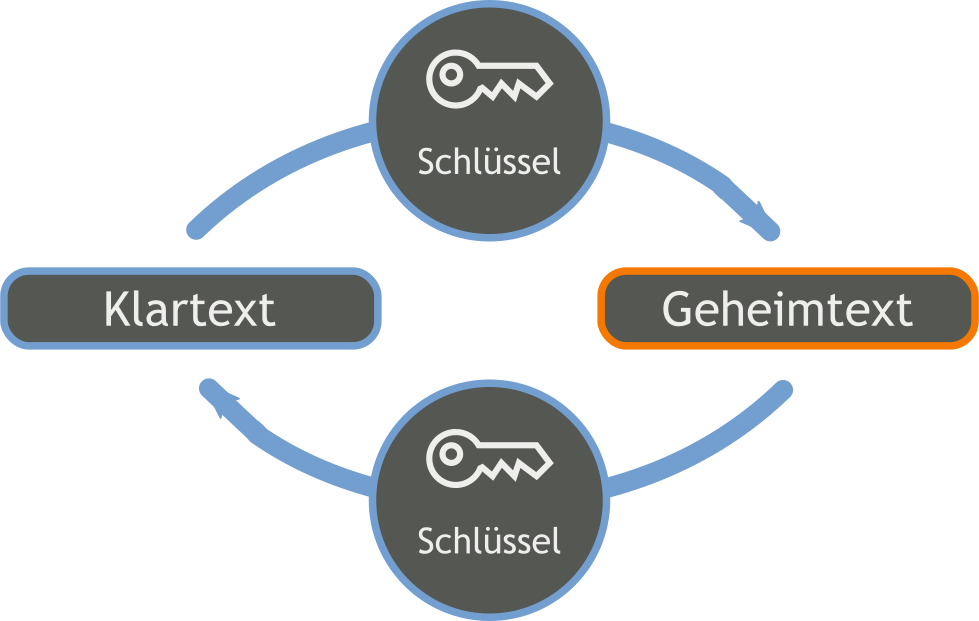
\includegraphics[width=0.5\textwidth]{images/Orange_blue_symmetric_cryptography_de.pdf}
  \end{center}
  \begin{itemize}
    \item Jahrtausende altes Konzept
    \item \emph{Ein} Schlüssel zum Ver- und Entschlüsseln,\\den \emph{alle} Beteiligten kennen
    \item Problem: Schlüsselaustausch
    \begin{itemize}
      \item Wer den Schlüssel kennt, kommt auch an die Daten
      \item Wer den Schlüssel kontrolliert, kontrolliert die Daten
    \end{itemize}
  \end{itemize}
  \tiny Bildquelle: \href{https://de.wikipedia.org/wiki/Datei:Orange_blue_symmetric_cryptography_de.svg}{,,Symmetrisches Kryptosystem'' von Bananenfalter / CC0}
\end{frame}

\begin{frame}{Asymmetrische Kryptographie}
  \begin{center}
    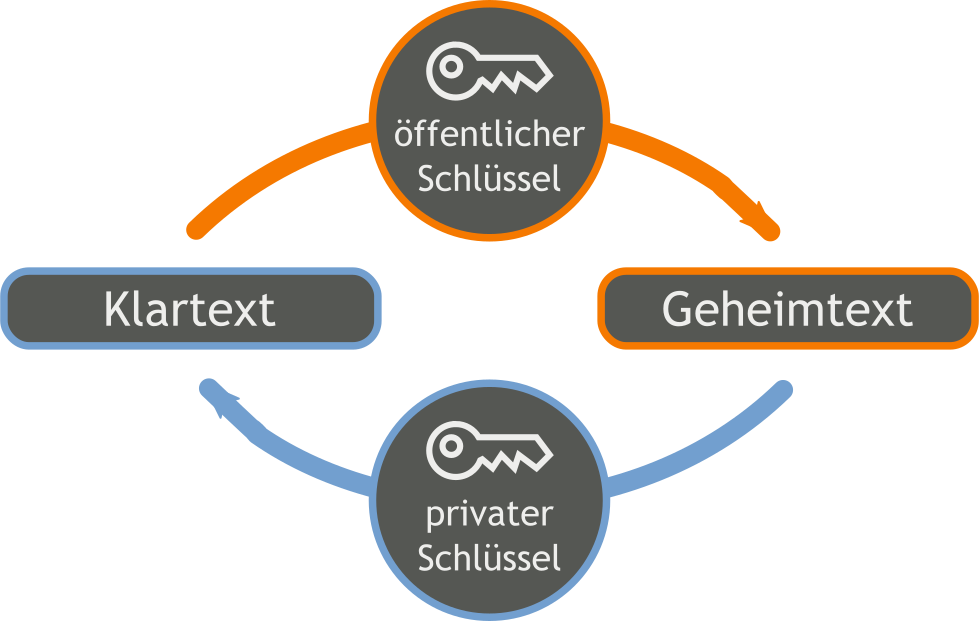
\includegraphics[width=0.5\textwidth]{images/Orange_blue_public_key_cryptography_de.pdf}
  \end{center}
  \begin{itemize}
    \item Prinzip: Schlüssel besteht aus einer \emph{privaten} und einer \emph{öffentlichen} ,,Hälfte``
    \begin{itemize}
      \item Öffentlichen Teil darf/muss man weitergeben
      \item Privaten Teil muss man unbedingt geheim halten
    \end{itemize}
    \item Wird verwendet, um vertraulichen Kanal aufzubauen
    \item Problem weiterhin: Authentizität des öffentlichen Teils
  \end{itemize}
  \tiny Bildquelle: \href{https://commons.wikimedia.org/wiki/File:Orange_blue_public_key_cryptography_de.svg}{,,Asymmetrisches Kryptosystem mit Verschlüsselung und Entschlüsselung'' von Bananenfalter / CC0}
\end{frame}

\begin{frame}{Asymmetrische Kryptografie -- Anwendungen}
  \begin{itemize}
    \item Verschlüsselung
      \begin{itemize}
        \item Absender \emph{verschlüsselt}\\ mit \emph{öffentlichem} Teil des \emph{Gegenübers}
        \item Nur Gegenüber\\ kann mit \emph{privatem} Gegenstück \emph{entschlüsseln}
      \end{itemize}
    \item Digitale Signatur
      \begin{itemize}
        \item Absender unterschreibt mit \emph{eigenem privaten} Teil
        \item Jeder kann mit \emph{öffentlichem} Gegenstück \emph{überprüfen}
      \end{itemize}
  \end{itemize}
  Es ist mathematisch komplex und benötigt Jahrtausende,\\ um aus einer Signatur oder dem öffentlichen Teil\\ den privaten Teil zu berechnen
\end{frame}

\endinput
